\begin{figure}
    \centering
    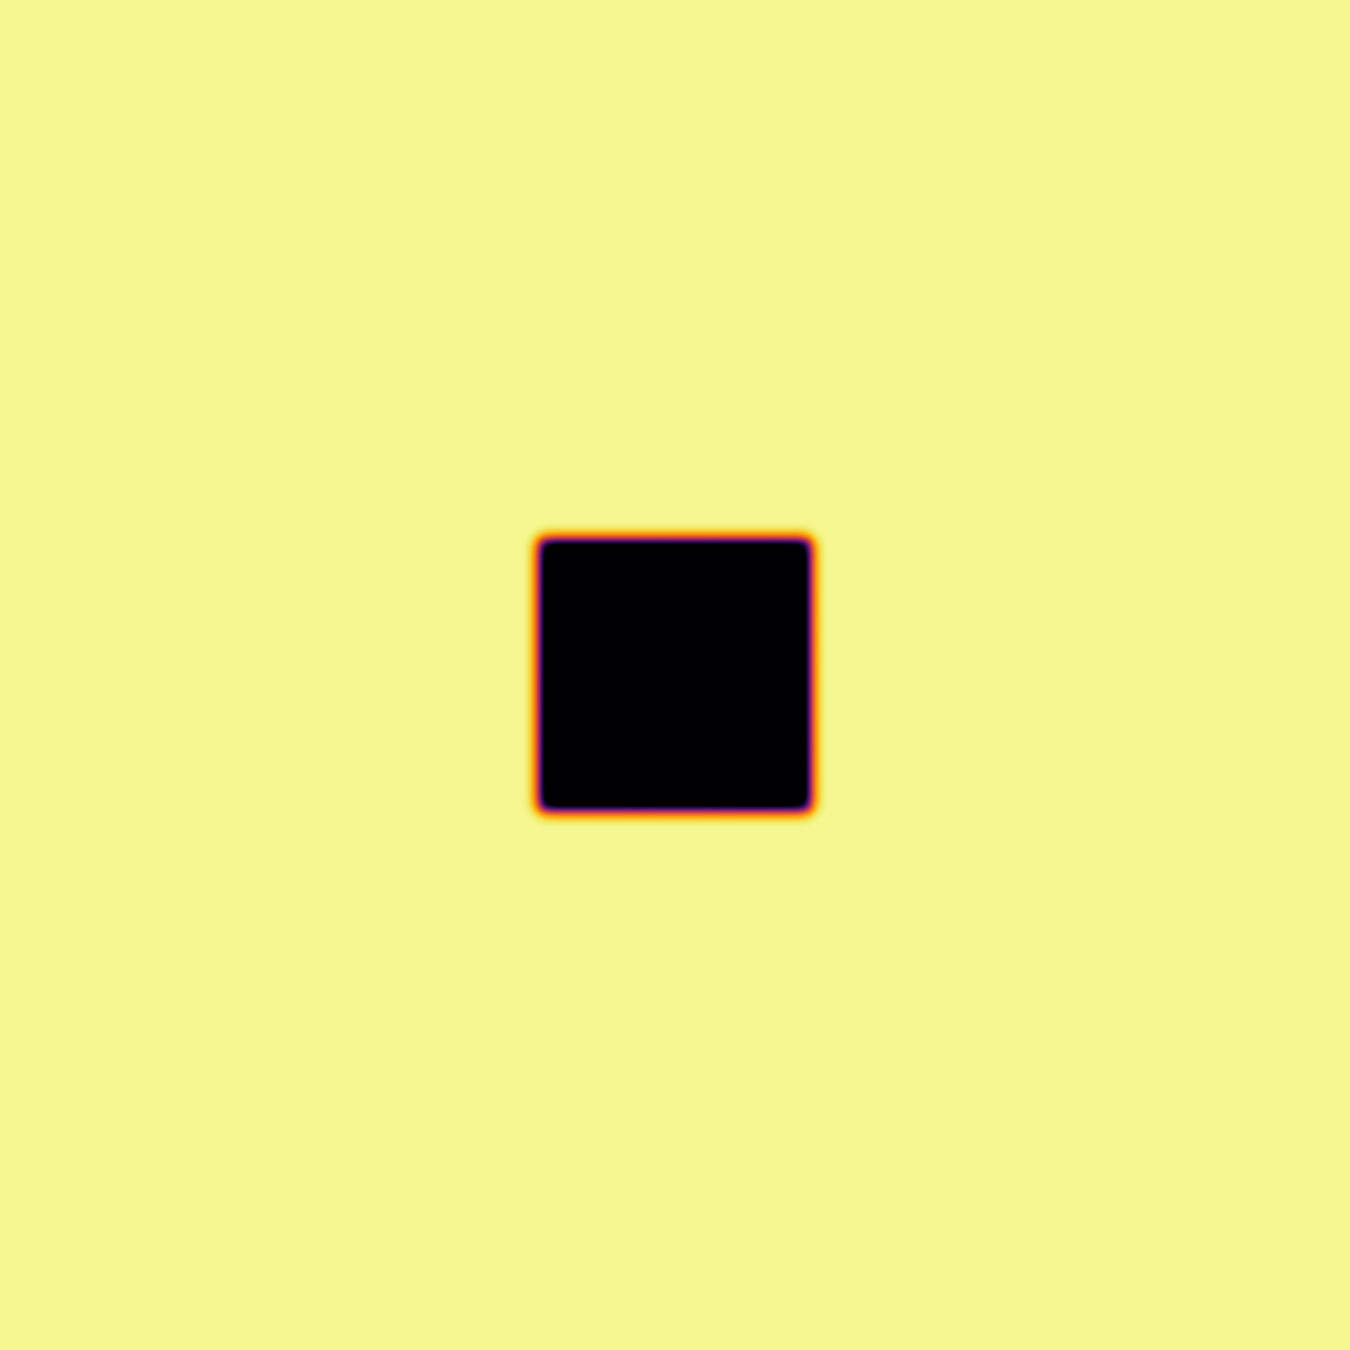
\includegraphics[width=0.32\linewidth]{papers/reaktdiff/images/GrayScott/gs_n1.png}
    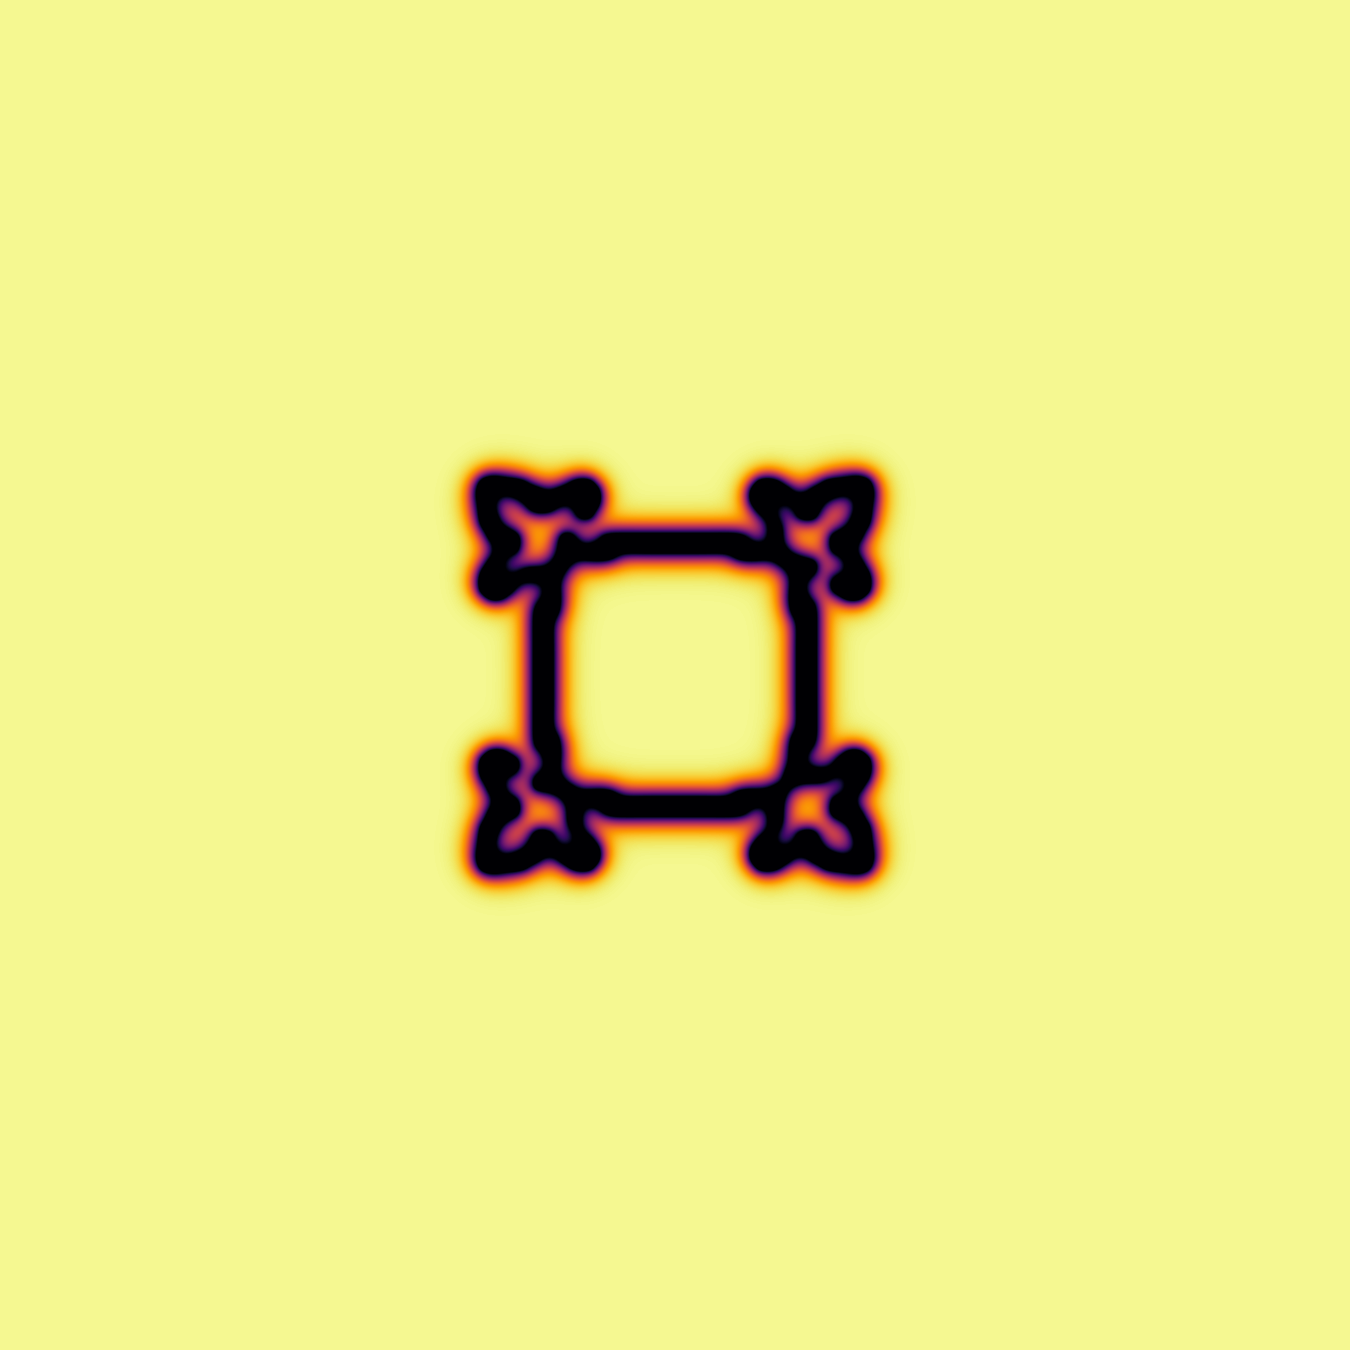
\includegraphics[width=0.32\linewidth]{papers/reaktdiff/images/GrayScott/gs_n300.png}
    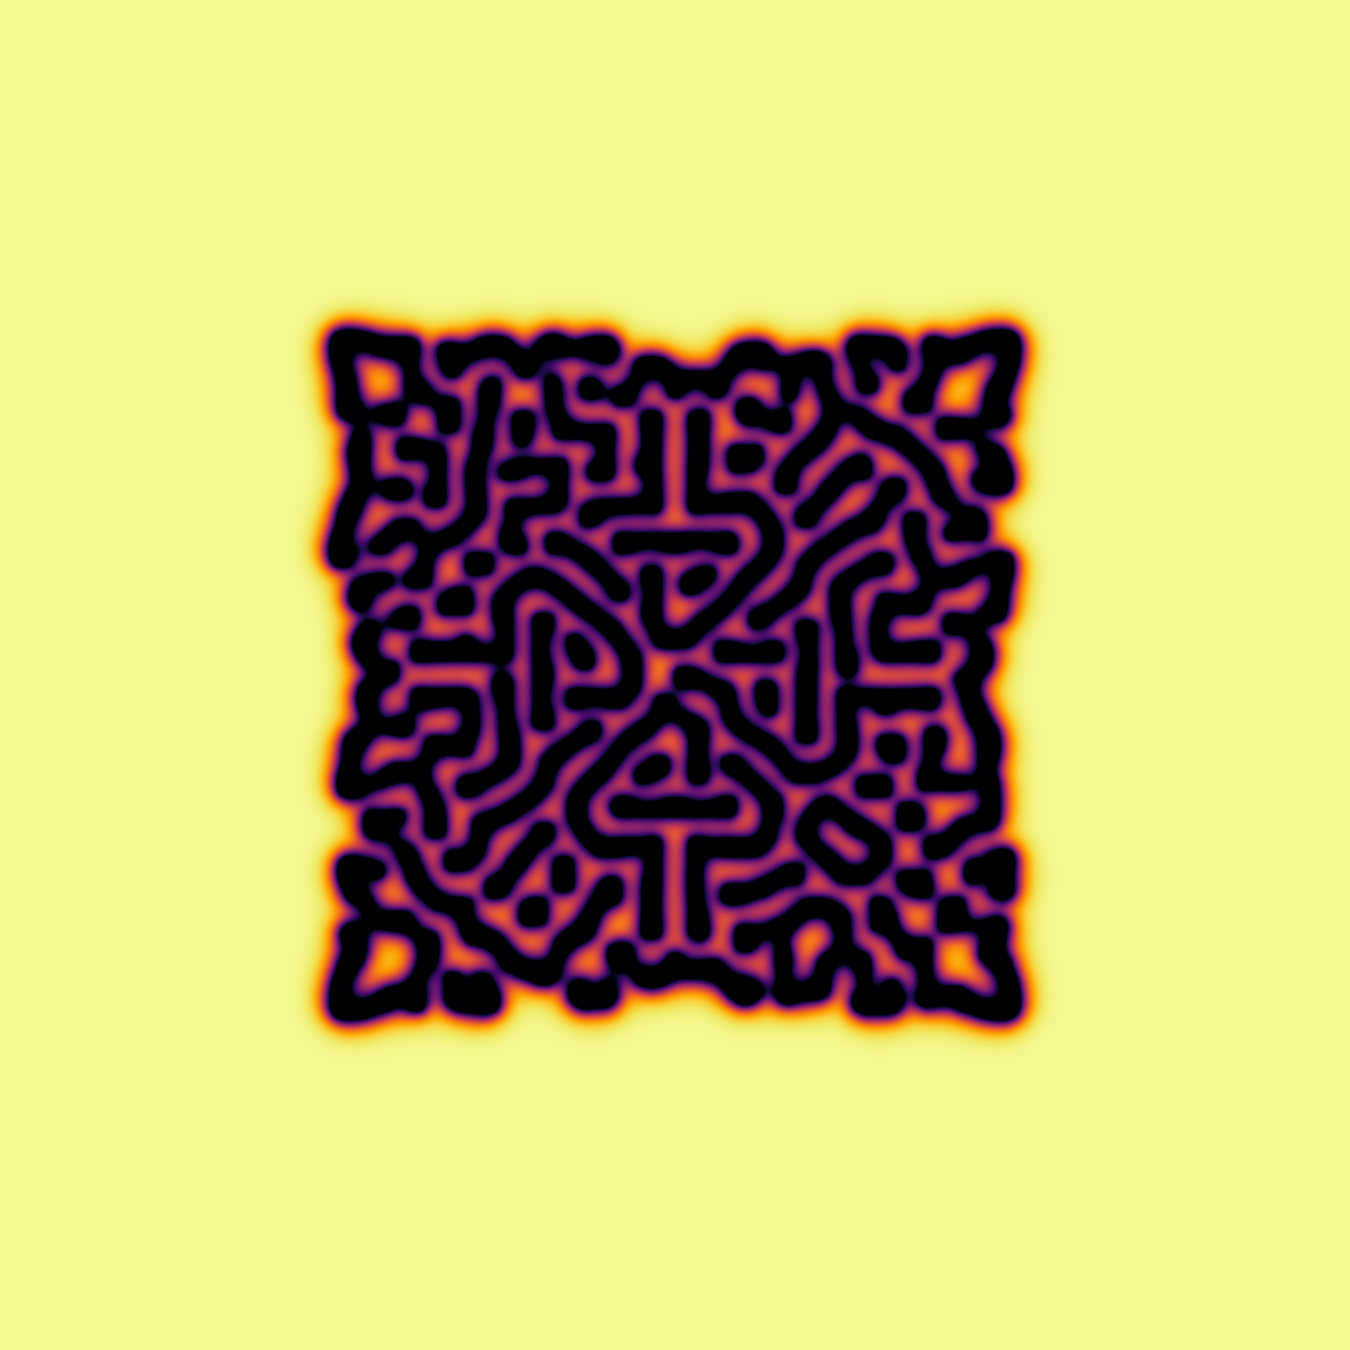
\includegraphics[width=0.32\linewidth]{papers/reaktdiff/images/GrayScott/gs_n999.png}
    \caption{Verlauf der Simulation (von links nach rechts) der Reaktions-Diffusiongleichung mit Gray-Scott-Modell (Gleichung \eqref{reaktdiff:equ:gs}) als Reaktionsterm.}
    \label{reaktdiff:fig:gs}
\end{figure}
